\section{Методы атомистического суперкомпьютерного моделирования} \label{part1_1_md}
\textit{Начало раздела \ref{part1_1_md} и раздел \ref{part1_1_md}.1 изложены согласно кандидатской диссертации автора \cite{shaytan_thesis_kfmn_2010} << }

О методах классического молекулярного моделирования написано множество подробных книг и монографий (см. например \cite{Frenkel,allen_computer_1989}), поэтому ниже мы лишь кратко обсудим основные понятия и подходы.

В основе методов классических атомистических методов молекулярного моделирования лежит представление о молекулярной структуре как о наборе классических частиц (материальных точек или в некоторых случаях твёрдых тел) взаимодействующих по законам классической механики. Молекулярно-механическая модель обычно предполагает следующие приближения: (i) электронные степени свободы не учитываются, а учитываются лишь атомные степени свободы, (ii) молекулы полагаются находящимися в основном энергетическом состоянии, (iii) автоматически предполагается приближение Борна-Оппенгеймера. На практике при задании конкретных типов взаимодействий между атомами в виде молекулярного гамильтониана предпринимается ещё ряд серьёзных приближений.

В случае моделирования биомолекулярных систем в приближении классической механики методические основы можно грубо разделить на три больших области: 1) задание механистической модели молекулярной системы на основе набора параметров, называемого силовым полем, 2) задание метода изучения динамики системы или метода изучения конформационного пространства данной системы, 3) различные технические и алгоритмические детали, связанные с эффективным и быстрым расчетом взаимодействий между атомами, а также оптимизацией расчетов на различных вычислительных системах.


%Ниже текст из файла materials/thesis_portable.pdf, ссылки надо смотреть там, но я их всех уже импортировал в зотеро.
%\todo{2S - из файла materials/thesis\_portable.pdf взять текст и картинки начиная со стр. 31 со слов "In molecular mechanics molecular system" до конца 39 страницы. с картинками и формулами. ссылки надо смотреть там, но я их всех уже импортировал в зотеро.}

\subsection{Силовые поля}
В молекулярной механике молекулярная система описывается в терминах классической механики набором точечных частиц (обычно представляющих атомы или группы атомов) и их взаимодействий, заданных функцией потенциальной энергии. Форма и структура функции потенциальной энергии называется силовым полем. На сегодняшний день разработано большое количество различных типов силовых полей, от обычных силовых полей до силовых полей, специфичных для определенного класса соединений. К наиболее популярным относятся группы силовых полей OPLS-AA \cite{jorgensen_development_1998}, AMBER \cite{cornell_2nd_1995}, CHARMM \cite{mackerell_all-atom_1998}, GROMOS \cite{schuler_improved_2001} , CVFF \cite{dauber-osguthorpe_structure_1988}, PCFF \cite{sun_force_1994}, MM3 \cite{allinger_molecular_1989} и другие. Эти силовые поля могут быть параметризованы относительно экспериментальных данных (в частности, калориметрических, спектроскопических), а также для воспроизведения поверхностей потенциальной энергии, вычисленных с помощью методов квантовой химии. Сложность функциональной формы силового поля может варьироваться, однако почти все молекулярные силовые поля содержат шесть общих основных термов для описания валентных и невалентных взаимодействий. Среди валентных взаимодействий выделяют термы описывающие растяжения ковалентных связей, деформации валентных углов, торсионных углов и ложноторсионные углы. Невалентные взаимодействия обычно описываются комбинацией парных ван-дер-Ваальсовых взаимодействий и кулоновских взаимодействий, основанных на точечных частичных зарядах атомов. Рисунок \ref{fig:p1_1:f10} и уравнение \ref{eq:p1_1:e1} дополнительно иллюстрируют эти термы. Многие из обычных силовых полей, используемых для моделирования биомолекул, включают в себя только упомянутые выше основные энергетические термины. Более сложные силовые поля (например, MM3, PCFF) могут также включать ангармонические члены и перекрестные члены для валентных взаимодействий, которые отражают связь между внутренними координатами. Например, при уменьшении валентного угла между атомами обнаруживается, что валентные связи удлиняются, чтобы уменьшить взаимодействие между атомами. Было обнаружено, что перекрестные члены играют важную роль в силовых полях, предназначенных для предсказания колебательных спектров  \cite{leach_molecular_2001}. Было высказано предположение, что наличие перекрестных членов (вместе с некоторыми другими особенностями) может обеспечить общий способ классификации силовых полей \cite{hwang_derivation_1994}. Согласно этой логике, силовое поле класса I ограничено гармоническими членами (например, для растяжения связей и валентного угла) и не имеет перекрестных членов. Силовое поле класса II будет иметь ангармонические члены и явные перекрестные члены для учета взаимоотношений между различными геометрическими параметрами. Еще одной характеристикой силового поля класса II считается возможность его использования без модификации одновременно для моделирования свойств изолированных малых молекул, конденсированных фаз и макромолекулярных систем \cite{leach_molecular_2001}.
\begin{multline}
    U(\{\vec{r}_i\})= \sum_{bonds} \frac{1}{2} k_b (l-l_0)^2  + \sum_{angels} \frac{1}{2}k_\theta (\theta - \theta_0)^2 + \sum_{torsions} \frac{1}{2} V_n [1+\cos({n\varphi-\varphi_0})] + \\
     \sum_{impropers} \frac{1}{2} k_\gamma (\gamma-\gamma_0)^2 + \sum_{j+1}^{N-1} \sum_{i=j+1}^{N} \Bigg\{ 4\epsilon_{ij} \Bigg[\Big(\frac{\sigma_{ij}}{r_{ij}}\Big)^{12} - \Big(\frac{\sigma_{ij}}{r_{ij}}\Big)^6\Bigg] + \frac{q_iq_j}{4\pi \epsilon_0 r_{ij}} \Bigg\} f_{ij}
     \label{eq:p1_1:e1}
\end{multline}

\begin{figure} [h!]
    \centering
    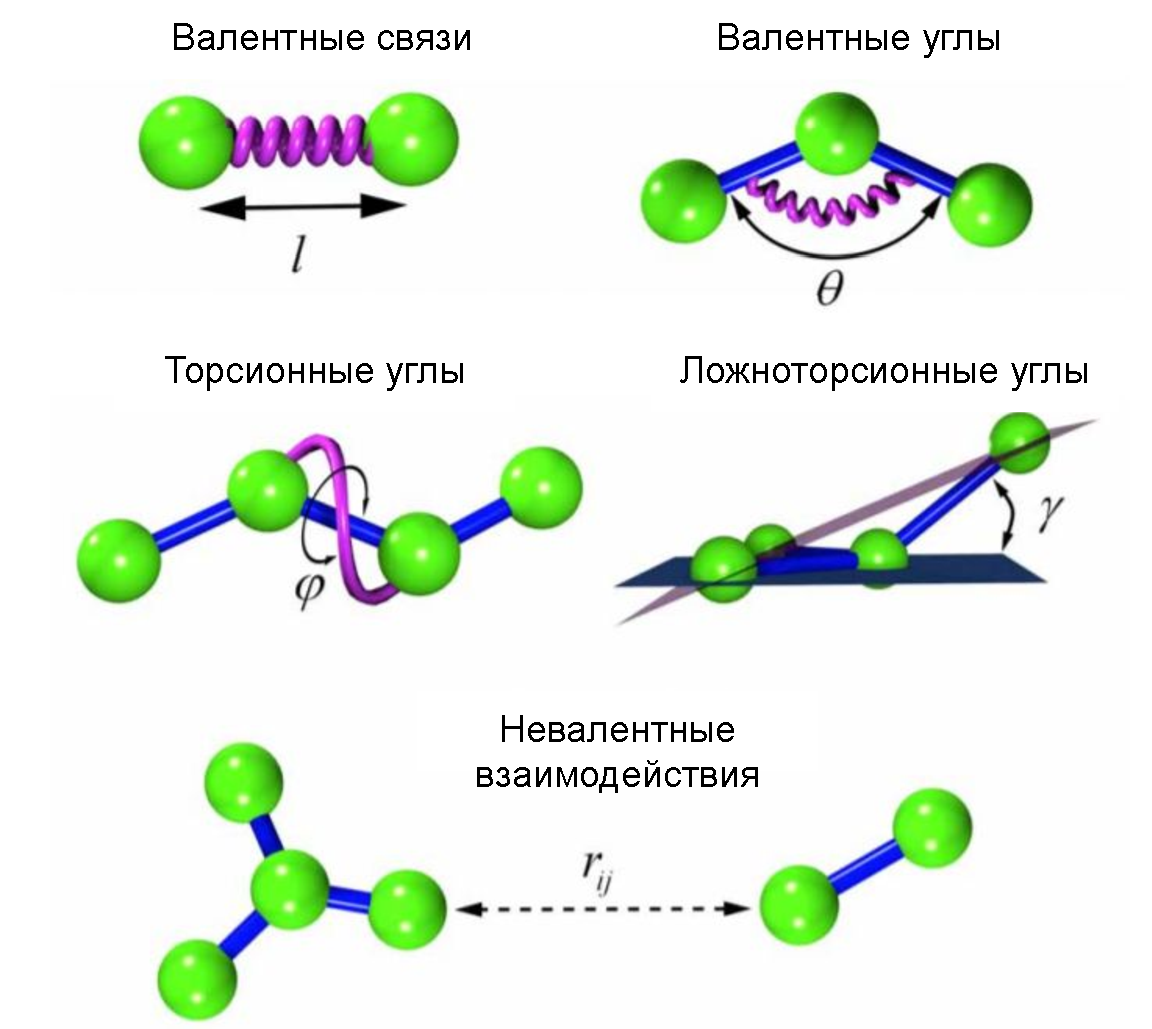
\includegraphics [width=\textwidth]{images/p1/part1_1_md/part1_1_md_f10.pdf}
    \caption[Энергетические термы силового поля]{Графическое изображение энергетических термов в силовых полях молекулярной механики. Атомы изображены зелеными сферами. Рисунок соответствует членам, представленным в уравнении 
    \ref{eq:p1_1:e1}}
    \label{fig:p1_1:f10}
\end{figure}


\subsubsection{Силовое поле OPLS-AA}
В качестве примера устройства типичного силового поля, применяемого для моделирования белков и других биологических молекул, рассмотрим поле OPLS-AA. Силовое поле OPLS-AA \cite{oplsaa,oplsaa2} является полноатомной версией поля OPLS (Optimized Potentials for Liquid Simulations), то есть атомы водорода рассматриваются явным образом. Параметры поля OPLS, в частности, подгонялись под экспериментальные свойства жидкостей, таких как плотность и теплота испарения.
Общая структура энергии молекулярной системы представлена в уравнении \ref{opls_ff_eqn}.

\begin{eqnarray}
&&U(r^N)=U_{bond}+U_{angle}+U_{dih}+U_{nb} \label{opls_ff_eqn}\\
&&U_{bond}=\sum_{bonds}K_r (r-r_{eq})^2\nonumber\\
&&U_{angle} = \sum_{angles} k_\theta \left ( \theta - \theta_{eq} \right )^2\nonumber\\
&&U_{dih} = \frac {V_1} {2} \left [ 1 + \cos \left ( \phi \right ) \right ] 
                + \frac {V_2} {2} \left [ 1 - \cos \left ( 2 \phi \right ) \right ] 
                + \frac {V_3} {2} \left [ 1 + \cos \left ( 3 \phi \right ) \right ] 
                + \frac {V_4} {2} \left [ 1 - \cos \left ( 4 \phi \right ) \right ]\nonumber\\
&&U_{nb}^{ab} = \sum_{i} ^{on\ a} \sum_{j} ^{on\ b} \left \{
                    4 \epsilon_{ij} \left [ \left( \frac {\sigma_{ij}}{r_{ij}} \right )^{12} 
                    - \left ( \frac {\sigma_{ij}}{r_{ij}} \right )^6 \right ]  + \frac {q_iq_j} {r_{ij}}
                   \right \} f_{ij}\nonumber
\end{eqnarray}
межмолекулярные взаимодействия $U_{nb}$ учитываются только для атомов, которые удалены на три и более связи, для 1-4 взаимодействий коэффициент скейлинга $f_{ij}=0.5$, во всех остальных случаях $f_{ij}=1$.

\subsubsection{Силовое поле PCFF}
Силовое поле PCFF (Polymer Consistent Force Field) \cite{pcff_sun_1994} основано на силовом поле CFF91 и относится к семейству силовых полей CFF (consistent force-field). Это поле создано для моделирования широкого класса органических полимеров, утверждается, что силовые поля второго поколения (к которым относится PCFF) более точно воспроизводят экспериментальные результаты, чем силовые поля первого поколения. Платой за это является более сложное устройство поля и наличие перекрёстных членов в функции энергии. Общий вид энергии молекулярной системы в приближении поля PCFF приведён в формулах \ref{pcff_eqn}. На Рис. \ref{fig:2_pcff_terms} приведено графическое пояснение к внутренним степеням свободы, являющимися параметрами для каждого члена потенциальной энергии.

\begin{eqnarray}
&&U(r^N)=U_{b}+U_{\theta}+U_{\phi}+U_{\chi}+U_{bb^\prime}+U_{\theta \theta^\prime}+U_{b\theta}+U_{b\phi}+U_{b^\prime \phi}+U_{\theta \phi}+U_{\phi \theta \theta^\prime}+U_{nb}  \nonumber \\
&&U_{b}=\sum_{b}K(b-b_0)^2\nonumber\\
&&U_{\theta}=\sum_{\theta}H(\theta-\theta_0)^2\nonumber\\
&&U_{\phi}=\sum_{\phi}V(1+\cos{(\phi-\phi_0)})\nonumber\\
&&U_{\chi}=\sum_{\chi}K_{\chi} \chi^2\nonumber\\
&&U_{bb^\prime}=\sum_{bb^\prime}F_{bb^\prime} (b-b_0)(b^\prime-b_0^\prime)\nonumber\\
&&U_{\theta\theta^\prime}=\sum_{\theta\theta^\prime}F_{\theta\theta ^\prime} (\theta-\theta_0)(\theta ^\prime-\theta _0^\prime)  \\  \label{pcff_eqn}
&&U_{b\theta}=\sum_{b\theta}F_{b\theta} (b-b_0)(\theta-\theta _0)\nonumber\\
&&U_{b\phi}=\sum_{b\phi}(b-b_0)[V_1\cos{\phi}+V_2\cos{2\phi}+V_3\cos{3\phi}]\nonumber\\
&&U_{b^\prime\phi}=\sum_{b^\prime\phi}(b^\prime-b^\prime_0)[V_1\cos{\phi}+V_2\cos{2\phi}+V_3\cos{3\phi}]\nonumber\\
&&U_{\theta\phi}=\sum_{\theta\phi}(\theta-\theta_0)[V_1\cos{\phi}+V_2\cos{2\phi}+V_3\cos{3\phi}]\nonumber\\
&&U_{\phi\theta\theta^\prime}=\sum_{\phi\theta\theta^\prime}K_{\phi\theta\theta^\prime}\cos{\phi(\theta-\theta_0)(\theta ^\prime-\theta _0^\prime)}\nonumber\\
&&U_{nb} = \sum_{i>j} \left \{ \left [ \frac { A_{ij} } { r_{ij}^9 } - \frac {B_{ij}} {r_{ij}^6} \right ]+ \frac{q_iq_j}  { r_{ij} } \right \} f_{ij}\nonumber
\end{eqnarray}

\begin{figure}[htbp]
  \centering
  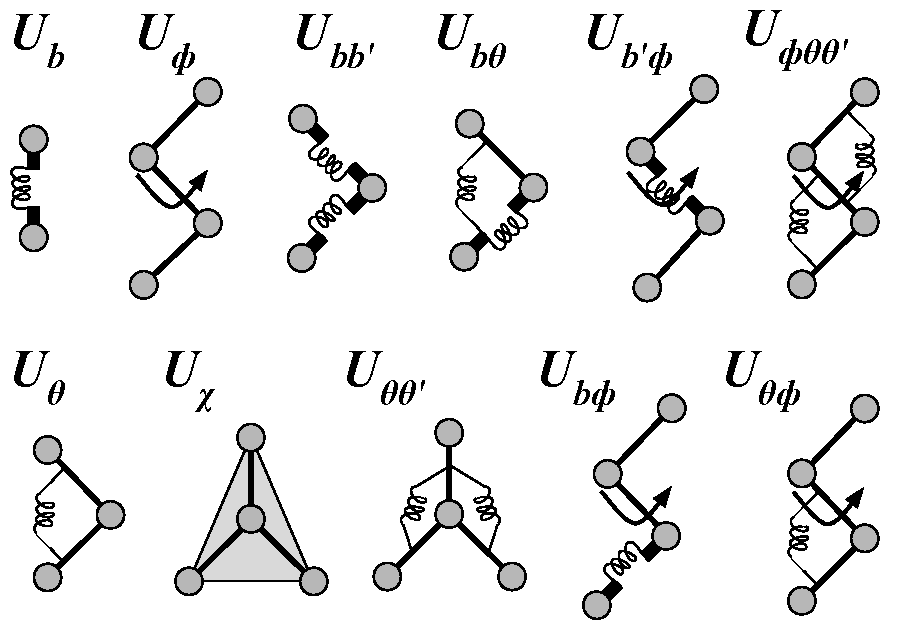
\includegraphics[width=15cm]{images/2_pcff_terms}
     \caption{Графическое пояснение к членам внутримолекулярной энергии уравнения \ref{pcff_eqn}.}
  \label{fig:2_pcff_terms}
\end{figure}

\textit{>>}

\subsection{Методы молекулярной динамики}

Определив модель молекулярной механики, можно применять различные методы для ее анализа; они включают в себя минимизацию энергии, моделирование молекулярной динамики, моделирование по методу Монте-Карло, а также различные более сложные методы, основанные на этих методах. Ключевым методом данной работы (а также, вероятно, наиболее часто используемым для изучения сложных молекулярных систем) является метод моделирования молекулярной динамики (МД) и его различных вариаций. Основная идея метода МД моделирования очень проста и основана на численном решении классических уравнений движения атомов в молекулярной системе на основе второго закона Ньютона:

\begin{equation}
    \frac{d^2 \overrightarrow{r_i}}{dt^2}= \overrightarrow{a}= \frac{\overrightarrow{F}}{m}= - \frac{1}{m_i} \nabla_i U(\textrm \{\vec{r_i}\})
\end{equation}
 
Численное решение обычно получается с помощью одной из схем интегрирования, такой как алгоритм Верле (velocity Verlet algorithm) \cite{swope_computer_1982}:

\begin{eqnarray}
    \overrightarrow{r}(t+\triangle t) = \overrightarrow{r}(t)+\overrightarrow{v}(t)\triangle t + \frac{1}{2} \overrightarrow{a}(t) \triangle t^2  \nonumber \\
    \overrightarrow{v}((t +\triangle t) =   \overrightarrow{v}(t) \frac{\overrightarrow{a}(t)+\overrightarrow{a}(t +\triangle t)}{2} \triangle (t)
\end{eqnarray}

Хотя основная идея, лежащая в основе МД-моделирования, на первый взгляд кажется довольно простой и понятной, ее обоснованность и интерпретация связаны с фундаментальными проблемами теоретической физики и математики на стыке механики, статистической физики и теории хаоса \cite{hoover_time_2001}. Одним из таких вопросов является связь между обратимыми во времени уравнениями Ньютона, используемыми для моделирования эволюции системы во времени, и эмпирическими необратимыми законами термодинамики, приводящими систему к состоянию, в котором энтропия максимальна.
    Другой набор вопросов и приближений, который имеет большое значение для практической реализации МД моделирования в реальных молекулярных системах, будет кратко обсужден ниже и включает использование периодических граничных условий, реализацию статистических ансамблей, динамику Ланжевена и диссипативных частиц, вычисления несвязанных взаимодействий, параллельная реализация МД алгоритмов.

\subsection{Периодические граничные условия}

Периодические граничные условия (ПГУ) - это метод, используемый для уменьшения влияния граничных эффектов на молекулярную систему во время моделирования и аппроксимации свойств объемных систем (таких как газы или жидкости) с помощью модели, состоящей из конечного набора молекул. Типичный случай применения периодических граничных условий - моделирование макромолекул в явном растворителе.
    В периодических граничных условиях ячейка моделирования окружена своими периодическими копиями во всех трех пространственных направлениях (см. Рисунок \ref{fig:p1_1:f11}), таким образом, эффективно образуя бесконечную кристаллическую структуру. Каждый атом, характеризуемый своими действительными координатами, также имеет координаты своих периодических образов. Распространенной формой учета частиц в периодических граничных условиях является соглашение о ближайшем образе, при котором каждый отдельный атом в системе взаимодействует с ближайшим к себе образом каждой частицы в системе.

\begin{figure} [h!]
    \centering
    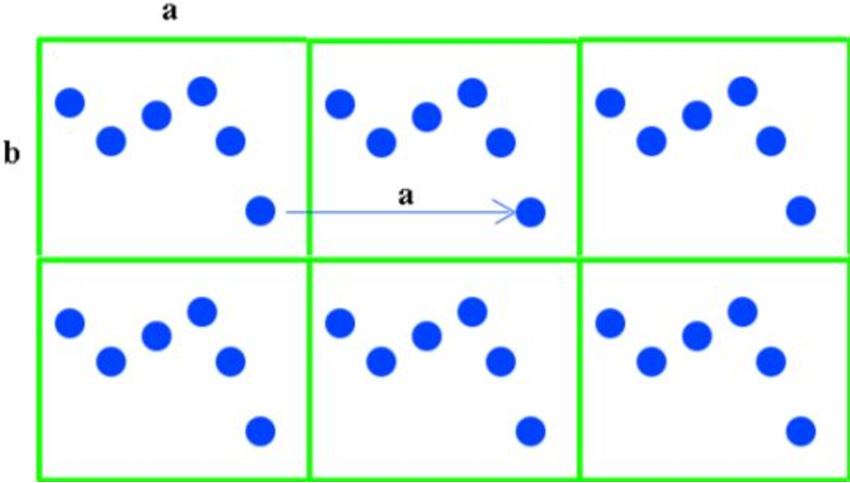
\includegraphics [width=\textwidth]{images/p1/part1_1_md/part1_1_md_f11.pdf}
    \caption[Иллюстрация периодических граничных условий]{Иллюстрация периодических граничных условий, используемых в МД моделировании. Кружками обозначены атомы и их периодические образы в соседних периодических ячейках.}
    \label{fig:p1_1:f11}
\end{figure}

ПГУ также используются в сочетании с методами учета электростатических взаимодействий на больших расстояния, такими как суммирование по Эвальду \cite{sagui_molecular_1999}. Поэтому полный электростатический заряд системы должен быть равен нулю, чтобы избежать проблем с расхождением значений полной электростатической энергии. Однако даже если система нейтральна, общий дипольный момент ячейки может приводить к некоторым искусственным энергетическим эффектам, похожим на пироэлектрические эффекты в полярных кристаллах.
Чтобы предотвратить артефакты связанные с ПГУ, размер ячейки моделирования должен быть достаточно большим, чтобы избежать таких нефизических эффектов. В том числе если размер ячейки слишком мал, макромолекула может взаимодействовать со своим собственным изображением в соседней ячейке, что эквивалентно взаимодействию молекулы с собой. Это может привести к нефизической динамике большинства макромолекул.

\subsection{Статистические ансамбли в МД моделировании}

Настоящие молекулярные системы никогда не изолированы от окружающей среды. Взаимодействие молекулярной системы с окружающей средой в плане обмена энергией, объемом и частицами с точки зрения статистической физики может быть описано в терминах статистических ансамблей \cite{landau_statistical_2000}. Ансамбль микросостояний молекулярной системы, связанной с внешним термостатом с постоянной температурой, называется каноническим ансамблем (или NVT-ансамблем), аналогично система под поршнем, связанная с термостатом, дает изобаро-изотермический ансамбль (или NPT -ансамбль).

    Поскольку базовые алгоритмы МД моделирования обеспечивают решение уравнений движения для изолированной системы (микроканонический ансамбль), обычно вводятся специальные алгоритмы, которые имитируют связь системы с внешним резервуаром энергии или объема \cite{frenkel_understanding_2002}. Цель таких алгоритмов - поддерживать правильные характеристики средней температуры (объема), в то же время обеспечивая правильную величину колебаний, которые зависят от внутренних свойств системы, таких как теплоемкость и сжимаемость.
    Среди алгоритмов термостатирования следующие алгоритмы нашли применение в современных кодах моделирования: термостат Берендсена \cite{berendsen_molecular_1984}, термостат Нозе-Гувера \cite{hoover_canonical_1985}, цепи Нозе-Гувера \cite{martyna_nose-hoover_1992}, термостат Андерсена \cite{andersen_molecular_1980}, термостат решкалирования скоростей \cite{bussi_canonical_2007}.
    
    Термостат Берендсена, будучи самым простым, полагается на масштабирование скоростей с коэффициентом $\lambda$  на каждом временном шаге:
\begin{equation}
   \lambda= \sqrt{\Big[1+\frac{\triangle t}{\tau_t} \Big\{\frac{T_0}{T}-1  \Big\} \Big]}
\end{equation}
    Влияние этого алгоритма на температуру заключается в том, что фактическая температура корректируется до эталонной температуры $T_0$ экспоненциальным образом:
\begin{equation}
    \frac{dT}{dt}= \frac{T_0 - T}{\tau}
\end{equation}
Однако термостат Берендсена имеет серьезные недостатки: во-первых, он не допускает колебаний температуры и, таким образом, не реализует правильный ансамбль, и, во-вторых, было показано, что процедура перемасштабирования скорости вызывает ``эффект летающего куба'' при моделировании системы в вакууме, когда энергия связанная с поступательным движением и вращением всей системы непрерывно растут, в то время как энергия высокочастотных основных мод истощается \cite{harvey_flying_1998,golo_dynamic_2002}.
    Формализм Нозе-Гувера - это подход, основанный на расширенном лагранжиане, содержащем дополнительные искусственные координаты и скорости, который приводит к детерминированной молекулярной динамике при постоянной температуре. Расширенный гамильтониан, первоначально предложенный Нозе \cite{nose_molecular_1984}, можно записать следующим образом:
\begin{equation}
    H_{Nose}= \sum_{i=1}^{N} \frac{\tilde {\mathbf p}_{i}^{2}}{2 m_i \tilde s^2} + U (\tilde r^N) + \frac{\tilde {\mathbf p}_{s}^{2}}{2Q} + g k T_0 ln(\tilde s)
\end{equation}
    где ${\mathbf p}_s$ и s - координаты расширенной переменной, Q - ее фиктивная масса, k - постоянная Больцмана, $T_0$-эталонная температура, g - параметр. Этот гамильтониан порождает микроканонический ансамбль из 6N + 2 степеней свободы. Переменные, присутствующие в этом гамильтониане, называются виртуальными переменными. Тем временем определяется набор реальных переменных, которые соотносятся с виртуальными переменными следующим образом:
\begin{eqnarray}
    {\mathbf r}= \tilde {\mathbf r} \\
    {\mathbf p}= \tilde {\mathbf p} /s \\
    s= \tilde s \\
    dt=d \tilde t / s
\end{eqnarray}
    и псевдогамильтониан может быть тогда задан как 
\begin{equation}
    H({\mathbf p},{\mathbf r})= \sum_{i=1}^{N} \frac{{\mathbf p}_{i}^{2}}{2m_i}+ U({\mathbf r}^N)
\label{pseudoH}
\end{equation}
Можно показать, что микроканонический ансамбль, сгенерированный путем решения уравнений движения для расширенной системы в виртуальных переменных, будет соответствовать канонической выборке реальных переменных согласно соответствующему псевдогамильтониану (\ref{pseudoH}), если параметр g = 3N и другие условия выполнены (см. ниже). Тепло передается в реальную систему и обратно от расширенной переменной колебательным образом, что приводит к почти периодическим колебаниям температуры. 
    Позже Нозе и Гувер показали, что соответствующие уравнения движения могут быть сформулированы в терминах реальных системных переменных, что дает уравнения движения Нозе-Гувера:
\begin{eqnarray}
    \ddot{{\mathbf r}_i} = \frac{{\mathbf F}_i}{m_i} - \frac{\xi \dot{{\mathbf r}_i}}{m_i} \nonumber \\
    \dot{\xi}= \frac{kg}{Q}(T(t)-T_0)
\end{eqnarray}

    Детальный теоретический анализ негамильтоновой динамики, генерируемой уравнениями Нозе-Гувера, показывает, что алгоритм генерирует правильное распределение только при наличии единственного интеграла движения, сохраняющегося во время динамики, обычно полной энергии расширенной системы, и никаких других интегралов движения \cite{frenkel_understanding_2002}. Исключением является сохранения полного импульса системы, если центр масс остается неподвижным.
    
    Данное утверждение также подразумевает, что динамика является эргодической, то есть усреднение по траектории эквивалентно усреднению по фазовому пространству. Однако было показано, что для небольших или жестких систем динамика неэргодична, и правильные распределения не генерируются. Чтобы решить эту проблему, Martyna et al. \cite{martyna_nose-hoover_1992} предложили схему, в которой термостат Нозе-Гувера соединен с другим термостатом или цепочкой термостатов.
    
    В подходе Андерсена к изотермическому моделированию система связана с термостатом с помощью стохастических импульсных сил, которые время от времени действуют на случайно выбранные частицы. В процессе столкновения частицы приобретают новые скорости согласно распределению Максвелла-Больцмана, соответствующие заданной температуре. Термостат Андерсена обеспечивает правильный статистический ансамбль, но делает динамику прерывистой из-за случайных столкновений.
    
    Термостат решкалирования скорости (Velocity rescale), предложенный Bussi et al. \cite{bussi_canonical_2007} представляет собой комбинацию термостата Берендсена со стохастическим членом, который обеспечивает правильное распределение кинетической энергии.
    
    
    Аналогично алгоритмам термостатирования существуют алгоритмы баростатирования, которые позволяют реализовать правильное целевое давление и NPT ансамбль. Схема баростатирования Берендсена \cite{berendsen_molecular_1984} позволяет быстро отрелаксировать систему до целевого давления и поддерживать его на протяжении всего моделирования. Алгоритм Берендсена изменяет масштаб координат и векторов ячейки моделирования на каждом шаге с помощью матрицы $\mu$ при заданном эталонном давлении $P_o$ следующим образом:
\begin{equation}
    \hat{\mu}_{ij}= \delta_{ij} - \frac{\triangle t}{3 \tau_p} \beta_{ij} \big\{P_{0ij}-P_{ij}(t)\big\}
\end{equation}
Где $\beta$ - изотермическая сжимаемость.
    Это приводит к экспоненциальной релаксации давления в соответствии с законом:
\begin{equation}
    \frac{dP}{dt}=\frac{P_0 -P(t)}{\tau_p}
\end{equation}
Как и в случае с термостатом, баростат Берендсена не полностью реализует NPT ансамбль и подавляет правильные флуктуации давления и объема, однако, если эти флуктуации не являются термодинамически значимыми, данный подход является простым и удобным методом поддержания постоянного давления в системе.

    Другой схемой поддержания давления, аналогичной термостату Нозе-Гувера, которая правильно реализует NPT ансамбль, является схема  Парринелло-Рамана \cite{parrinello_polymorphic_1981}.

\subsection{Ланжевеновская и диссипативная динамика частиц}
    Ланжевеновская (или стохастическая) динамика и диссипативная динамика частиц (ДДЧ) (dissipative particle dynamics) - это методы, которые позволяют имитировать влияние растворителя на динамику молекулярной системы посредством введения диссипативных и стохастических членов в уравнения движения. Взаимодействие диссипативных и стохастических сил не только изменяет динамику, но также может гарантировать правильные характеристики NVT ансамбля. В пределе небольшого воздействия (малая вязкость растворителя) эти методы также являются удобными алгоритмами для поддержания NVT ансамбля при моделировании методом МД.
    
    
    Стохастическая или скоростная динамика Ланжевена добавляет трение и шум к уравнениям движения Ньютона следующим образом:
\begin{equation}
   m_i \ddot{{\mathbf r}}={\mathbf F}_i - m_i \xi_i \dot{{\mathbf r}} + \hat{{\mathbf r}_i}
   \label{eq:p1:langevin}
\end{equation}
    где $\xi_i$ - постоянная трения, а $\hat{r_i}(t)$ - это шумовой процесс с корреляционной функцией
\begin{equation}
   \big  \langle \hat{r}_{i}^{\alpha}(t)\hat{r}_{i}^{\beta}(t+s) \big \rangle = 2m_i \xi_i kT \delta(s) \delta_{ij} \delta_{\alpha\beta}
   \label{eq:p1:lang_proc}
\end{equation}
т.е. он нескоррелирован для разных частиц, разных компонентов и разного времени. Формальный вывод уравнения Ланжевена посредством редукции быстрых степеней свободы и их аппроксимации двумя последними членами уравнения (\ref{eq:p1:langevin}) основан на технике проекционного оператора, введенной Мори и Цванцигом \cite{zwanzig_nonequilibrium_2001}. В остальном члены, отвечающие за трение и стохастический процесс, имеют интуитивно понятный физический смысл: первая представляет собой диссипативную силу, вызываемую трением с растворителем, вторая - своего рода движущую силу, которая вызывается ``ударами'' окружающих частиц растворителя.

Случайное трение и стохастические силы не сохраняют ни импульс, ни энергию системы. Под действием силы трения энергия отводится из системы, в то время как стохастический процесс может закачивать энергию в систему, поэтому динамика и выборка больше не соответствуют микроканоническому ансамблю, в то время как энергия системы флуктуирует, что напоминает канонический ансамбль NVT. Кроме того, можно показать, что для реализации распределения Больцмана в стохастической динамике трение и стохастические силы должны быть связаны через уравнение (\ref{eq:p1:lang_proc}).
        
Хотя метод Ланжевена привлекателен для жидкостных систем, где структура растворителя не важна, или как алгоритм для строгой реализации ансамбля NVT, он не дает правильной гидродинамики, поскольку случайные силы и силы трения не сохраняют импульс системы. Чтобы преодолеть эту проблему, но при этом сохранить положительные черты стохастической динамики, метод диссипативной динамики частиц (ДДЧ) (dissipative particle dynamics) был первоначально разработан Хугербрюгге и Кольманом для мезоскопического моделирования простых и сложных жидкостей \cite{hoogerbrugge_simulating_1992}. В ДДЧ сила, действующая на каждую частицу, состоит из трех членов \cite{moeendarbary_dissipative_2009}:
\begin{equation}
    {\mathbf F}_i= \sum_{j \neq i} ({\mathbf F}_{ij}^{C} + {\mathbf F}_{ij}^{D} +{\mathbf F}_{ij}^{R})
\end{equation}
консервативная сила, диссипативная сила и случайная сила, соответственно. В то время, как консервативная сила является обычной парной силой, диссипативная и случайная силы определяются следующим образом:
\begin{equation}
   {\mathbf F}_{ij}^{D} = -\gamma \omega_D (r_{ij})({\mathbf n}_{ij} \cdot {\mathbf v}_{ij}) {\mathbf n}_{ij}
\end{equation}
\begin{equation}
   {\mathbf F}_{ij}^{R}= \sigma \omega_R (r_{ij}) \zeta_{ij} {\mathbf n}_{ij}
\end{equation}
где $r_{ij}= |{\mathbf r}_i -{\mathbf r}_j|$j, ${\mathbf n}_{ij}= {\mathbf r}_{ij}/|{\mathbf r}_{ij}|$, $\gamma$ и $\sigma$ - скалярные параметры, представляющие силу трения и случайную силу. $\omega_D$ и $\omega_R$ - весовые коэффициенты, которые варьируются от 0 до 1 и исчезают выше радиуса отсечки $R_c$. $\zeta_{ij}$ - представляет собой гауссовский белый шум со следующими свойствами:
\begin{equation}
   \big\langle \zeta_{ij}(t) \big\rangle = 0, \zeta_{ij}=\zeta_{ji}
\end{equation}
\begin{equation}
    \big\langle \zeta_{ij}(t) \zeta_{i' j'}(t') \big \rangle= \big( \delta_{ii'}\delta_{jj'}+\delta_{ij'}\delta_{i'j} \big) \delta(t-t')
\end{equation}
Замечательной особенностью уравнений ДДЧ в отличие от динамики Ланжевена является то, что
диссипативные и случайные силы зависят только от относительного положения и скорости
частицы и действуют по векторам, соединяющим пары частиц. Это в сочетании с
симметрией индексов обеспечивает выполнение третьего закона Ньютона и сохранение количества движения. Далее можно показать, что уравнения ДДЧ описывают
системы в ансамбле NVT при $\sigma^2 = 2\gamma kT$. Выбор одной весовой функции может
быть произвольным, однако можно показать, что обе функции должны быть связаны как
$\omega_D (r) = (\omega_R (r))^2$.
Типичный выбор для этой функции:
\begin{equation}
    \omega (r)= \Bigg\{ 2 \bigg(1- \frac{r}{R_c}    \bigg), r \leq R_c  ;   0, r > R_c\Bigg\}
\end{equation}
ДДЧ в основном применяется как метод мезоскопического моделирования, где частицы ДДЧ представляют собой целые молекулы или области жидкости, а не отдельные атомы. Однако трение и случайные члены могут также использоваться в атомистическом моделировании для моделирования влияния растворителя и реализации ансамбля NVT. Преимуществами термостата ДДЧ перед термостатом Ланжевена является сохранение импульса и малый радиус взаимодействий ДДЧ, оба фактора способствуют крупномасштабным конформационным переходам в молекулярной системе, если они должны произойти.

\subsection{Расчет невалентных взаимодействий}
    Вычисление невалентных взаимодействий и особенно кулоновских взаимодействий - одна из задач МД моделирования. Важной отличительной чертой электростатических взаимодействий является их медленный затухающий характер $(\sim 1/r)$, что, строго говоря, делает некорректным обрезку электростатического взаимодействия на некотором расстоянии во время вычисления сил и энергии при моделировании. В трехмерной объемной системе энергия взаимодействия точечной частицы с окружающей средой, характеризуемой плотностью заряда $\rho (r)$, была бы выражена интегралом:
\begin{equation}
   E= \iiint \frac{\rho (\vec{r})}{|\vec{r}- \vec{r}_0|} d^3 \vec{r}
\end{equation}
    который может сходиться только условно. Таким образом, необходимо соблюдать особую осторожность при расчете электростатических взаимодействий в моделировании МД. Было показано, что при простой обрезке кулоновских взаимодействий могут возникать серьезные артефакты, особенно при моделировании систем зарядов, начиная от шума и нестабильности при моделировании и заканчивая неблагоприятным воздействием на молекулярный порядок \cite{sagui_molecular_1999}.
    Если изучаемая система не является периодической (т.е. не используются периодические граничные условия), единственной альтернативой полному расчету электростатических взаимодействий (что для больших систем является недопустимо дорогостоящим, поскольку масштабируется как $\sim N^2)$ является их обрезка на некотором расстоянии Rc. Однако необходимо обосновать отсутствие серьезных побочных эффектов в таком случае. Наиболее распространенные ошибки могут возникать из-за: (i) отсутствия непрерывности силы, особенно при образовании нескомпенсированных зарядов на длине радиуса обрезания, приводящего к алгоритмическому шуму и тепловыделению, (ii) для заряженных систем и систем с внутренней периодичностью энергия и поведение системы могут зависеть от радиуса обрезания причудливым образом.
    
    В системах, которые используют периодические граничные условия, может использоваться альтернативная более надежная стратегия суммирования электростатических взаимодействий, она основана на методе суммирования Эвальда и родственных алгоритмах PME (particle mesh Ewald) и PPPM (particle-particle particle-mesh Ewald), основанные на интерполяции функций по значениям в узлах сеток \cite{frenkel_understanding_2002}. Идея суммирования по Эвальду состоит в том, чтобы заменить бесконечную медленно сходящуюся сумму электростатического взаимодействия данного набора частиц и всех их периодических образов двумя быстро сходящимися суммами, одна в прямом, а другая - в обратном пространстве. Рассмотрим представление набора точечных зарядов, дополненных гауссовыми функциями экранирования и их обратными функциями на рисунке \ref{fig:p1_1:f12}.

\begin{figure} [h!]
    \centering
    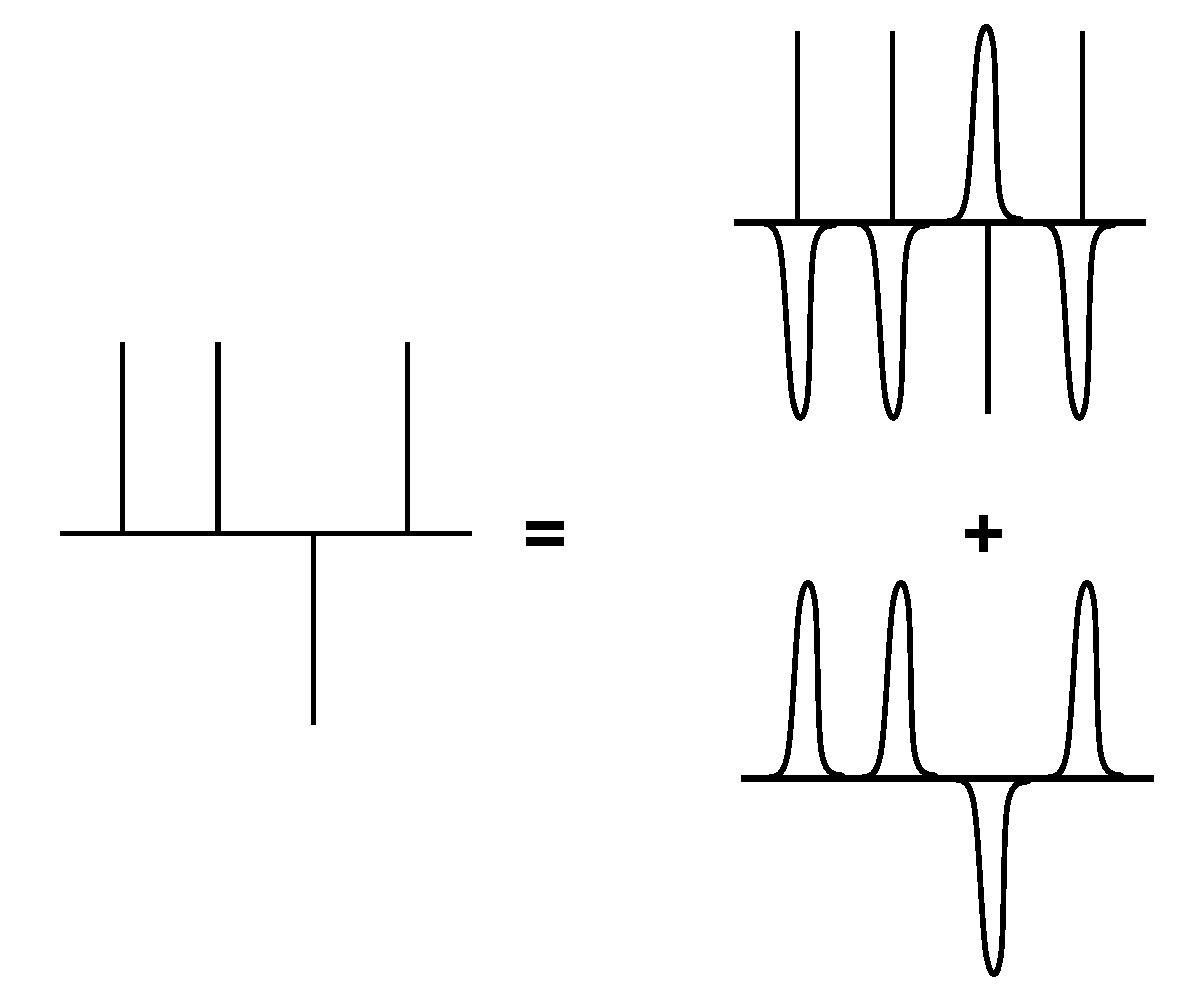
\includegraphics [width=\textwidth]{images/p1/part1_1_md/part1_1_md_f12.pdf}
    \caption{Схематическое изображение разложения заряда, используемого в суммировании по Эвальду.}
    \label{fig:p1_1:f12}
\end{figure}

    Гауссовские экранирующие функции имеют вид:

\begin{equation}
    \rho_{Gauss}(r)= -q_i(\alpha/\pi)^{3/2} exp(-\alpha r^2)
\end{equation}
    Можно показать, что в этом случае полный электростатический потенциал может быть выражен как сумма потенциалов обеих подсистем, представленных на рисунке \ref{fig:p1_1:f12}, за вычетом члена энергии самовзаимодействия. Электростатический потенциал экранированных точечных зарядов быстро спадает и может быть суммирован в прямом пространстве, в то время как потенциал компенсирующей подсистемы (плавно меняющиеся периодические гауссианы) можно легко вычислить в обратном пространстве Фурье на основе решения уравнения Пуассона. Результирующая полная энергия системы может быть записана следующим образом:
\begin{equation}
    U= \frac{1}{2} \sum_{i \neq j}^{N} \frac{q_i q_j \erfc{(\sqrt{\alpha}r_{ij})}}{r_{ij}} + \frac{1}{2V} \sum_{k \neq 0}\frac{4 \pi}{k^2} |\rho ({\mathbf k})|^2 exp(-k^2 / 4\alpha) - (\alpha/ \pi)^{1/2} \sum_{i=1}^{N} q_{i}^{2}
\end{equation}
    где $\rho ({\mathbf k}) \equiv \sum_{i=1}^{N} q_i exp(i{\mathbf k} \cdot {\mathbf r}_i)$, V - объем периодической ячейки.

    Однако сумма Эвальда требует больших вычислительных ресурсов для больших систем с порядком масштабирования  $O(N^{3/2})$ и остается дорогостоящей по сравнению с традиционными схемами обрезки взаимодействий. Чтобы решить эту проблему, были разработаны подходы на основе интерполяционных сеток, все они пытаются ускорить решение уравнения Пуассона в периодических граничных условиях, используя преимущества быстрого преобразования Фурье (БПФ) для вычисления дискретных преобразований Фурье \cite{sagui_molecular_1999}. Эти методы могут масштабироваться как $O(N log (N))$.
    Методы суммирования, подобные суммированию по Эвальду, могут вычислять электростатическую энергию в периодической системе с заданной точностью. Их использование привело к значительному повышению стабильности при моделировании биомолекул. Однако, некоторые фундаментальные проблемы моделирования все еще существуют и могут привести к артефактам во время моделирования \cite{sagui_molecular_1999}. Смит и Петтитт \cite{smith_ewald_1996,smith_presence_1997} изучали динамические артефакты, вызванные суммированием по Эвальду. Они сосредоточились на вопросе о величине энергетических барьеров при свободном вращении диполей в системах с периодичностью (наличием дальнего порядка). Представьте себе единственный идеальный диполь в начале элементарной ячейки, который затем периодически воспроизводится в соседних ячейках. Потенциальная энергия системы будет зависеть от ориентации диполя, что не подходит для исследования растворов биомолекул. Однако Смит и Петтитт показали, что вращательные барьеры незначительны для дипольных молекул в растворителях с высокой диэлектрической проницаемостью при комнатной температуре с типичными размерами ячейки моделирования. Для моделирования в растворителях с низкой диэлектрической проницаемостью или в вакууме отсутствие артефактов не может быть гарантированно.






% \subsection{Методы молекулярной динамики}
% Задача молекулярной динамики фактически заключается в решении классических уравнений движения для системы с заданным гамильтонианом. Решение уравнений движения реализуется численно с помощью разностных схем таких, как алгоритм Верле или Лип-Фрог алгоритм. Важной особенностью ``хороших'' алгоритмов является обратимость во времени и сохранение объёма фазового пространства. Известно также, что алгоритм Верле обладает ``теневой'' характеристикой, то есть точки траектории, получаемые посредством этого алгоритма, точно соответствуют (конечно, за исключением ошибки численного округления) некоторой ``теневой траектории'' механической системы, которая однако не проходит, через точку с начальными условиями. Иными словами, алгоритм Верле генерирует траекторию, которая соответствует экстремуму действия для некоторой ``теневой траектории'' (\cite{Frenkel} разд. 4.3.5).

% Для решения проблемы поверхностных эффектов в методе МД применяют периодические граничные условия. Особое внимание в последнее время обращается на тот факт, что при использовании периодических условий необходимо использовать решёточные алгоритмы для учёта дальнодействующих взаимодействий, таких как электростатические, поскольку обрезание зарядовых взаимодействий может приводить к артефактам моделирования. На данный момент хорошо разработаны достаточно быстрые решёточные алгоритмы учёта электростатики такие, как методы PME и PPPM.

% Отдельной проблемой является задание ансамблей в методе молекулярной динамики. Для задания распределения по температуре существует два принципиальных подхода: стохастическая и негамильтонова динамика. В стохастическом подходе в уравнения движения вводятся случайные члены (например, такие как в уравнении Ланжевена), которые позволяют привести статистическое распределение точек МД траектории к каноническому ансамблю. Подход негамильтоновой динамики был предложен Гувером \cite{Hoover}, он разработал такую модификацию уравнений движения, в которой предельным для точек фазового пространства является каноническое распределение. Однако в оригинальном алгоритме Нозе-Гувера были найдены проблемы при некоторых условиях, и на данный момент наиболее надёжным считается алгоритм цепей Нозе-Гувера.

